\documentclass[10pt]{article}
\usepackage[margin=1in]{geometry}
\usepackage[T1]{fontenc}
\usepackage{lmodern}
\usepackage{microtype}
\usepackage{graphicx}
\usepackage{booktabs}
\usepackage{amsmath,amssymb}
\usepackage{caption}
\usepackage{xcolor}
\usepackage{tcolorbox}
\usepackage{enumitem}
\usepackage[hidelinks]{hyperref}
\captionsetup{font=small,labelfont=bf}
\setlist{itemsep=1pt,topsep=3pt}

\newtcolorbox{tech}[1][]{colback=gray!6,colframe=gray!45,boxrule=0.4pt,arc=1pt,left=5pt,right=5pt,top=3pt,bottom=3pt,
  fonttitle=\small\bfseries,title={Technical details#1},coltitle=black,colbacktitle=gray!18}

\title{Can a Decision Model Play a Market Participant?\\[3pt]
\large Jev in the card game Figgie, compared with the rule-based traders of Ozerov et al.}
\author{Jace Yang\\\small\url{https://github.com/jaceyang97/figgie-on-jev}}
\date{26 September 2026}

\begin{document}
\maketitle

\begin{abstract}
\noindent
Jev is a decision model. It reads a description of a situation and gives a probability for each option in a list.
We test whether Jev can play the part of a known type of market trader. We use Figgie, a small card game that copies a
trading floor, and the rule-based traders of Ozerov, DiSilvio and Luo (2021). We use two sets of market rules: the
paper's order book (A) and the real game's open outcry (B). The study has three stages. Stage~0 replicates the paper
with rule-based traders only. Stage~1 asks Jev about 1,200 frozen game moments (4,700 requests). Stage~2 puts Jev in
full games: 26 conditions, 40 games each, and each game is paired with a game in which the rule-based ``twin'' sits
in the same seat with the same cards (\STAGETWOREQUESTS{} requests). Main results: (1)~In the paper's 240-second
setting, the rule-based traders rank as in the paper (fundamentalist, then bottom-feeder, then noise trader); in the
paper's 10,000-event setting, the bottom-feeder beats the fundamentalist in 2 of 4 line-ups. (2)~Jev's belief about the
goal suit is worse than the card-counting calculation and than a uniform guess, and Jev is most wrong when it is most
sure. (3)~A persona text moves Jev's actions toward the twin in 22 of 24 cells, but the similarity stays low
(0.04--0.57). (4)~\STAGETWOABSTRACT{}
\end{abstract}

\section{Introduction}

Many people now ask whether AI models can stand in for people in economic experiments. For chat models, this idea has a
name: \emph{homo silicus} (Horton, 2023). Jev is a different kind of model. It does not write text. It reads a state
and a list of options, and it returns a probability for each option. This makes it easy to use as a trader in a
simulated market: at each moment, the options are the legal actions.

We ask a simple question: \emph{if we tell Jev which type of trader to be, does it act like that trader, and does it
earn what that trader earns?} To answer it, we need traders whose behaviour is exactly known. The Figgie study of
Ozerov, DiSilvio and Luo (2021) gives four such traders, with full algorithms. We add two market makers from the
literature. Each rule-based trader is a \emph{twin}: the reference that Jev must copy.

We have four research questions. We wrote them, and our predictions, before we collected the data.
\begin{itemize}
\item \textbf{RQ1, belief.} How well does Jev estimate the goal suit?
\item \textbf{RQ2, market rules.} How do rule sets A and B change the results?
\item \textbf{RQ3, persona wording.} Can a text description control Jev's actions? Which type of description works better?
\item \textbf{RQ4, profit.} Does Jev make more or less money than its twin in the same seat?
\end{itemize}
We fixed three primary measurements in advance: the change in similarity to the twin that each persona causes (decision
layer), the difference in log loss between Jev and card counting (belief), and the mean profit difference between Jev
and its twin in each rule set (game layer). All other results are secondary.

\section{The game and the model}

\paragraph{Figgie.} The deck has 40 cards in four suits. One suit has 12 cards, one has 8 and two have 10. No player
knows which suit has how many. The \emph{goal suit} is the suit of the same colour as the 12-card suit; it has 8 or 10
cards. Each of four players starts with 350 chips, pays 50 into a pot of 200 and gets 10 cards. For 4 minutes, the
players buy and sell cards for chips. At the end, each goal-suit card pays 10 chips from the pot, and the player with
the most goal-suit cards gets the rest of the pot (100 or 120 chips; a tie splits it). Profit is final chips minus
starting chips (350). The game is zero sum.

\paragraph{Jev.} Jev (\texttt{typesafe/jev-1.13}, served as \texttt{typesafe/jev-1.13-20260917}) reads a JSON state
of up to 64,000 tokens and answers one or more questions. A \emph{choice} question has up to 255 options, each with a
one-line description. Jev returns a probability for every option. We call it through OpenRouter. Input costs US\$0.042
per million tokens; output is free.

\begin{tech}
\small
There are 12 possible decks (3 choices of the 12-card suit's partner position $\times$ 4 suits, Table~1 of the paper).
A request is \texttt{\{model, state, questions\}}. Each question has a \texttt{type}, an instruction text and, for
\texttt{choice}, a map from option label to description. The answer holds \texttt{choice} (the most probable label) and
\texttt{probabilities} (all labels). We never use Jev's own \texttt{choice} field; we sample (section~\ref{sec:jev}).
\end{tech}

\section{Method}

\subsection{The simulator}
The simulator is event driven, as in the paper. Each trader wakes after a random gap (exponential, mean $1/\lambda$).
It looks at the market and decides. If it sends an order, the order reaches the market $\Lambda$ seconds later, and the
trader wakes again only after that. A game lasts 240 seconds, or, in the paper's setting, 10,000 events.

\paragraph{Two rule sets.}
\begin{itemize}
\item \textbf{A, order book} (the paper's Algorithm~1). Many orders can wait at each price. A new order trades with the
best waiting order on the other side, at the waiting order's price. Other orders stay after a trade. A player keeps at
most 5 orders per side and suit (the oldest goes). A player can cancel its orders in a suit.
\item \textbf{B, open outcry} (the real game). Each suit has one best bid and one best ask. A new bid must be higher than
the best bid; a new ask must be lower than the best ask. Every trade removes all bids and asks in all suits.
\end{itemize}

\paragraph{Speed.} In stages 1 and 2, all traders, Jev included, wake 0.5 times per second on average and their orders
arrive 0.3 seconds later (the \emph{equal speed}). So a profit difference cannot come from speed. For the replication,
we also use the paper's speed (1 wake per second, no delay).

\begin{tech}
\small
\textbf{Latency.} The paper sends an order $2\Lambda$ after the moment the trader sees the market (its method~(b)). Our
parameter is this total delay, so the paper's slow traders ($\Lambda = 100$) have a delay of 200.
\textbf{Order book details.} Price--time priority; self-trade prevention (a trader's own opposite order is removed, not
filled); an order whose owner can no longer pay or deliver is removed when it reaches the top. The paper trades at the
buy order's price; we trade at the waiting order's price, which is the standard rule in real order books.
\textbf{Common random numbers.} Game $g$ has seed $s(g)$. The seed fixes the deal and one random stream per seat for
wake-up gaps and for the trader's own random choices. So game $g$ has the same cards, in the same seats, in every
condition, and the opponents' streams are the same in the Jev arm and in the twin arm.
\end{tech}

\subsection{The rule-based traders}
All four traders of the paper send orders with the same rule (the paper's Algorithm~2): pick buy or sell with equal
chance; to buy, draw a price between 0 and the buy value; to sell, draw a price between the sell value and twice the
sell value; take the standing price if it is better. The traders differ only in how they value a suit.
\begin{itemize}
\item \textbf{Fundamentalist.} Values a suit from \emph{card counting}: the cards it knows exist (its hand, plus cards
it saw others sell), the probability of each of the 12 decks, and the payout of one more card, including its share of
the majority prize. It deletes its orders that no longer agree with its values (the paper's Algorithm~4).
\item \textbf{Bottom-feeder.} Copies the fundamentalists: its value is the middle of their last 4 buy and last 4 sell
prices. In stages 1 and 2, it never copies the seat under test, so the opponents act the same in every condition.
\item \textbf{Chartist.} Expects the recent price trend to continue (Chiarella, Iori and Perell\'o, 2009).
\item \textbf{Noise trader.} Values a suit at the best bid times $e^Z$, $Z \sim N(0,1)$.
\item \textbf{Market maker, Glosten--Milgrom (GM)} (1985). Quotes the expected card value after a buy (ask) and after a
sell (bid), from card counting and the direction of other traders' trades. Never takes another trader's order.
\item \textbf{Market maker, Avellaneda--Stoikov (AS)} (2008). Quotes around the market price, moves the quotes against
the cards it holds, and quotes wider when prices move a lot and early in the game. Never takes another trader's order.
\end{itemize}

\begin{tech}
\small
\textbf{Fundamentalist value} (paper, section~2.3): $e_b(j,n,m) = \sum_i m_i\, v(i,j,n)$ with $v = 0$ if $j$ is not the
goal suit of deck $i$, else $10 + v_m(i,n)$; $v_m(i,n) = a_i r^n$ for $n < x_i$, else 0, with $r = 1.2$,
$a_i = p_i(1-r)/(1-r^{x_i})$, $x_i \in \{5,6\}$ the majority size and $p_i \in \{120,100\}$ the prize.
$e_s(j,n,m) = e_b(j,n-1,m)$.
\textbf{GM:} belief $\pi_s \propto \mathrm{cc}_s \cdot \prod$ trade-flow likelihoods with a share $\mu = 0.3$ of
informed traders; ask $= 10\,\pi(1+\mu)/(\pi(1+\mu)+(1-\pi)(1-\mu))$, bid with $\mu \to -\mu$.
\textbf{AS:} reservation price $r = \text{mid} - q\gamma\sigma^2\tau$, half spread
$\gamma\sigma^2\tau/2 + \ln(1+\gamma/k)/\gamma$, with $\gamma = 0.1$, $k = 1.5$, $q$ = cards held minus cards dealt,
$\sigma^2$ from trade-price changes, $\tau$ = share of the game left.
\end{tech}

\subsection{The Jev trader}\label{sec:jev}
At each wake-up, the Jev trader sends one request with two questions: ``which action?'' and ``which suit is the goal
suit?''. The request has four parts.
\begin{enumerate}
\item \textbf{Rules.} A short text with the correct rules of Figgie and of the rule set. It has no strategy hints.
\item \textbf{State.} Hand, chips, time left, the order book (A: best 3 prices per side and its own orders; B: best bid
and ask), and the version of the context under test: \emph{basic} (only this), \emph{+summary} (facts computed from
the public record: trade counts and last prices per suit, each player's net buys and sells, and Jev's own recent
actions and their results) or \emph{+log+summary} (also the full list of trades). Two further versions add values
that code calculates, and we use them only as tests: \emph{+known} (cards known to exist) and \emph{+assist} (the
card-counting probabilities).
\item \textbf{Persona.} None (\emph{neutral}), the \emph{algorithm} wording (the twin's steps, as text) or the
\emph{behaviour} wording (what the trader does, without steps or numbers).
\item \textbf{Actions.} Pass; take the best bid or ask; cancel (A only); or bid or ask at a price from a ladder of 30
prices (1--20, then 22--40 in steps of 2). This gives at most 253 options.
\end{enumerate}
Jev's action is a random draw from its probabilities (\emph{sampling}). The earlier study took the most probable option
and always chose a bid, because the bid had the most options. Sampling keeps Jev's randomness, which the persona
algorithms need.

\subsection{The three stages}
\paragraph{Stage 0: replication (free).} The paper's line-ups (figures 3--5, tables 2--3), 100 games each, in three
settings: A with 10,000 events, A with 240 seconds, and B with 240 seconds; each at the paper's speed and at the equal
speed. We also measure the profit noise of each trader in the stage~2 line-up.

\paragraph{Stage 1: decision layer (4,700 requests, US\$1.02).} We play rule-based games in the stage~2 line-up and
copy the tested seat's view at random wake-ups: 100 \emph{frozen moments} per rule set and trader type (at most 3 per
game, only where the twin can act). For each moment we know the true goal suit, the card-counting probabilities and the
twin's action distribution (4,000 draws of its random choices). Then:
\begin{itemize}
\item \textbf{1a, persona wording} (3,600 requests): each moment with the algorithm persona, the behaviour persona and
no persona, state version +summary.
\item \textbf{1b, state versions and belief} (1,000 requests): the fundamentalist seat's moments, no persona, all five
state versions.
\item \textbf{1c, repeatability} (100 requests): 50 moments asked twice.
\end{itemize}

\paragraph{Stage 2: game layer (\STAGETWOREQUESTS{} requests, US\$\STAGETWOCOST{}).} One seat is Jev; the other three
are a fundamentalist, a bottom-feeder and a noise trader (the paper's line-up types; the chartist loses so much that it
would give free profit to the others). There are 26 conditions: 2 rule sets $\times$ (neutral $+$ 6 types $\times$ 2
wordings). Each condition plays 40 games, fixed in advance. Each condition has a twin arm: the rule-based trader of the
same type in the same seat and games (the twin of neutral is the fundamentalist). Seats rotate from game to game.

\begin{tech}
\small
\textbf{Similarity.} For Jev's distribution $\pi$ and the twin's $\tau$ over the menu,
$\mathrm{overlap} = \sum_a \min(\pi(a), \tau(a)) = 1 - \mathrm{TV}(\pi,\tau)$. ``Actions only'' renormalises both
without pass. A twin price outside the ladder moves to the nearest ladder price (3.1\% of the twin's probability mass).
\textbf{Belief.} Log loss $-\ln p(\text{goal})$ (primary; uniform $= \ln 4 \approx 1.386$), Brier score
$\sum_s (p_s - \mathbb{1}[s = \text{goal}])^2$ (uniform $= 0.75$), top-1 accuracy, calibration.
\textbf{Game layer.} $d_g = \text{profit}_{\text{Jev}} - \text{profit}_{\text{twin}}$ in the same seat and seed. We
fit $d_g = \beta_0 + \beta_A\mathbb{1}[A] + \beta_D\mathbb{1}[\text{behaviour}] + \beta_{AD}\mathbb{1}[A]\mathbb{1}[\text{behaviour}]
+ \sum_k \gamma_k \mathbb{1}[\text{type} = k] + \varepsilon_g$, and again with the number of goal cards in the starting
hand as a covariate.
\textbf{Uncertainty.} All 95\% intervals come from a cluster bootstrap over games (4,000 resamples; 1,000 for the
regression). In stage~1, the 24 persona-versus-neutral comparisons get a Holm correction.
\textbf{Selection rule for stage 2.} Use the cheapest factual state version whose log loss is not clearly worse than the
best one (paired 95\% interval includes 0).
\end{tech}

\section{Results}

\subsection{Stage 0: replication}

Figure~\ref{fig:rep} compares our rule-based games with the paper's figures 3--5.

\begin{figure}[t]
\centering
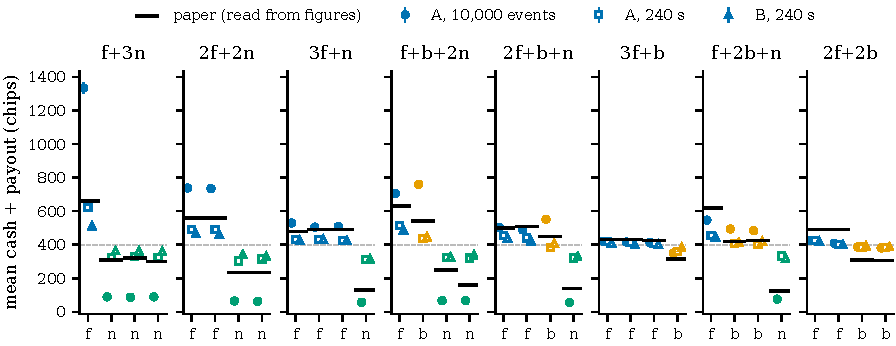
\includegraphics[width=\linewidth]{figures/stage0_replication.pdf}
\caption{Mean cash $+$ payout per seat (the paper's measure; profit $+$ 400), 100 games per line-up, paper's speed.
Black bars: values read from the paper's figures (approximate). Error bars: $\pm 2$ SE. f = fundamentalist,
b = bottom-feeder, n = noise trader. The dashed line (400) is the break-even value.}
\label{fig:rep}
\end{figure}

\begin{itemize}
\item \textbf{The fundamentalist wins in every line-up and every setting}, and the noise trader loses, as in the paper.
The more fundamentalists in a game, the less each one earns, as in the paper.
\item \textbf{The order f $>$ b $>$ n holds in all four bottom-feeder line-ups in both 240-second settings} (A and B,
both speeds). In the 10,000-event setting, the bottom-feeder earns more than the fundamentalist in two line-ups
(f+b+2n: 360 vs 306 chips; 2f+b+n: 152 vs 96). So hypothesis H2a holds for 240-second games only.
\item \textbf{Our profits are larger than the paper's in the 10,000-event setting and smaller in the 240-second
setting.} In 10,000 events, our noise traders lose almost all their chips (final cash about 14 of 300). The paper's
figures fall between our two settings.
\item \textbf{Homogeneous games (the paper's table 2).} Four fundamentalists: SD of final wealth, cash and payout
57.8, 30.0 and 67.8 (paper: 61.8, 33.1, 68.6). Four bottom-feeders: no trades (paper: no trades). Four noise traders:
\emph{no trades} (paper: SD of cash 188.5). The paper does not say what a noise trader does when a suit has no bid;
in our reading of the paper it has no value and does not trade, so a market of noise traders never starts.
\item \textbf{Latency (the paper's table 3).} One fast fundamentalist (delay 0) against three slow ones (delay 200):
each slow trader ends with more cash than the fast one (+47 to +51 chips; paper +58 to +66) and less payout ($-33$ to
$-39$; paper $-20$ to $-50$). The wealth difference (+10 to +14) has the paper's sign (+12 to +41), but its interval
includes 0.
\item \textbf{Rule set B} makes trade rarer (for f+3n: 35 vs 114 trades per game in A) and halves the fundamentalist's
advantage (112 vs 222 chips), as predicted (H2b).
\end{itemize}

\begin{table}[h]
\centering\small
\begin{tabular}{lcccc}
\toprule
 & \multicolumn{3}{c}{95\% interval, slow minus fast (chips)} \\
Competitor & Wealth & Cash & Payout \\
\midrule
slow0 & [-8.2, 36.9] & [39.8, 54.1] & [-56.3, -8.9] \\
slow1 & [-8.8, 33.3] & [43.5, 57.3] & [-60.2, -16.2] \\
slow2 & [-11.4, 32.0] & [41.2, 53.9] & [-59.9, -15.0] \\

\midrule
Paper, slow0 & [15.7, 38.4] & [58.1, 65.8] & [$-$46.8, $-$23.0] \\
\bottomrule
\end{tabular}
\caption{Latency test (A, 10,000 events, 100 games), as the paper's table 3.}
\end{table}

\paragraph{Noise check for stage 2.} In the stage~2 line-up at equal speed, the SD of the profit difference between two
rule-based types in the same seat and games is 62--97 chips. With 40 games, this gives a minimum detectable difference
of 28--43 chips per condition (Table~\ref{tab:noise}, appendix).

\subsection{Stage 1: decisions at frozen moments}

\paragraph{Belief (RQ1).} Figure~\ref{fig:ll} and Table~\ref{tab:1b} show the goal-suit belief.
\begin{itemize}
\item \textbf{Jev is worse than card counting} in every state version (log loss difference +0.17 to +0.28 in A and
+0.21 to +0.26 in B), and \textbf{worse than a uniform guess} (1.47--1.65 vs 1.386). H1a is not supported. The best
version is +log+summary in A (1.47; its interval against card counting just includes 0).
\item \textbf{Card counting itself is weak}: log loss 1.30 in A and 1.40 in B, close to the uniform 1.386. The paper's
calculation uses few facts, and our moments come from all game times.
\item \textbf{Jev is most wrong when it is most sure} (Figure~\ref{fig:cal}). When Jev gives a suit 0.4--0.6, that suit
is the goal suit only 8--15\% of the time.
\item \textbf{With the card-counting probabilities in its state (+assist), Jev becomes too confident} (H1b supported).
Its mean top probability rises to 0.69, much higher than the 0.49 of the numbers it was given, and its log loss rises
to 1.95 (A) and 1.80 (B), although its top-1 accuracy rises to the level of card counting (0.45 and 0.37).
\item \textbf{Later moments are not clearly better} (H1c): with +summary, log loss falls from 1.55 to 1.48 in A and
rises from 1.57 to 1.69 in B (earlier vs later half of moments).
\item \textbf{State version for stage 2.} Against the best factual version (+log+summary), +summary is not clearly worse
(A: +0.043, interval [$-$0.006, 0.091]; B: +0.011, [$-$0.037, 0.057]); basic is clearly worse in A (+0.092,
[0.007, 0.183]). By the rule we fixed in advance, stage~2 uses +summary (about 5,700 tokens per request in A and 4,900
in B).
\end{itemize}

\begin{figure}[t]
\centering
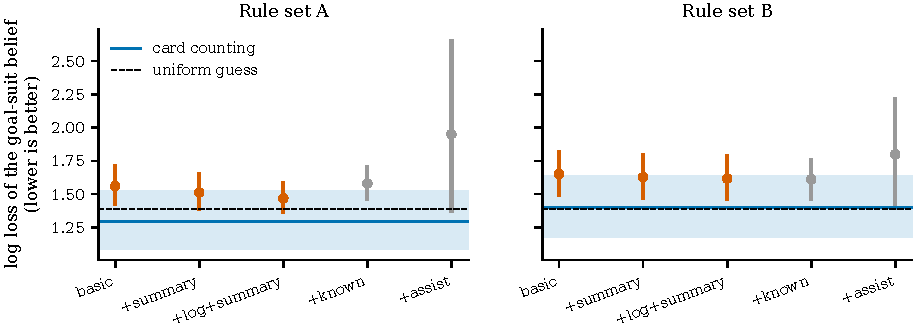
\includegraphics[width=0.78\linewidth]{figures/stage1_logloss.pdf}\hfill
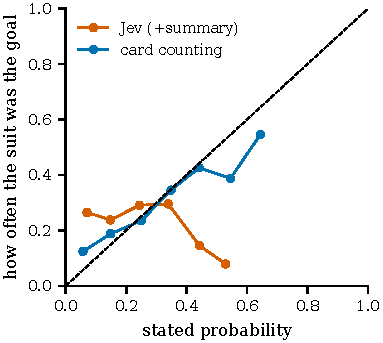
\includegraphics[width=0.21\linewidth]{figures/stage1_calibration.pdf}
\caption{Left: log loss of Jev's goal-suit belief for five state versions (100 fundamentalist moments per rule set;
95\% intervals). Grey: versions with values calculated by code (tests only). Blue line and band: card counting at the
same moments. Right: calibration of the +summary version, both rule sets (400 suit probabilities per curve).}
\label{fig:ll}\label{fig:cal}
\end{figure}

\paragraph{Persona wording (RQ3).} Figure~\ref{fig:ov} shows the similarity between Jev and the twin.
\begin{itemize}
\item \textbf{A persona moves Jev toward the twin in 22 of 24 cells} (Holm-corrected). The gains are 0.01--0.21. Two
cells move away: the algorithm fundamentalist in B ($-0.035$) and the behaviour noise trader in B ($-0.063$).
\item \textbf{The similarity stays low.} The best cells are the noise trader (0.55, algorithm, both rule sets) and the
bottom-feeder in B (0.57). The fundamentalist, the type with the most calculation, reaches only 0.36--0.43 (H3b
supported: Jev does not do the calculation).
\item \textbf{The market makers are almost never matched} (0.04--0.10), because their twin posts one precise price per
side and Jev spreads its probability over many prices. Jev also takes other traders' orders 1--14\% of the time,
although both market-maker personas say ``never take'' (H3a only partly supported; the rule is obeyed better in B).
\item \textbf{The words can act literally} (H3c). The behaviour noise-trader text says ``you take the current best bid
as a loose anchor''. In B, Jev then buys with 57\% of its probability, while the twin buys 8\% (Figure~\ref{fig:sh}).
\item \textbf{Neither wording is better overall,} and the effect of the wording is different in A and B (H3d not
supported): the algorithm wording gives the higher similarity for 5 of 6 types in A but only 2 of 6 in B.
\end{itemize}

\begin{figure}[t]
\centering
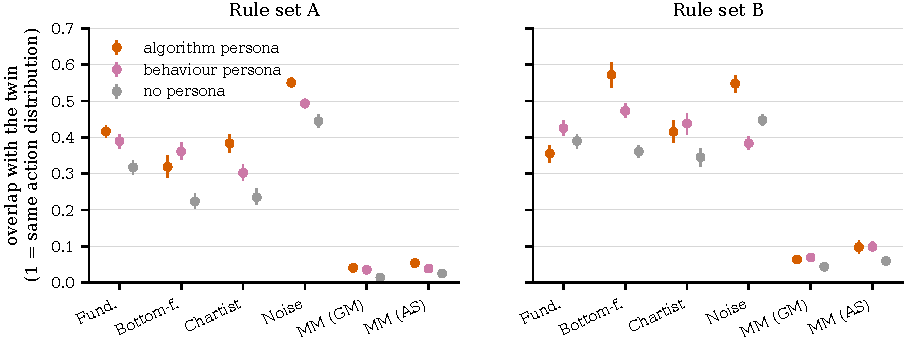
\includegraphics[width=\linewidth]{figures/stage1_overlap.pdf}
\caption{Similarity (overlap) between Jev's action distribution and the twin's, 100 moments per point, 95\% intervals.}
\label{fig:ov}
\end{figure}

\paragraph{Repeatability.} The same request gives almost the same answer: over 50 moments asked twice, the mean total
variation distance is 0.071 for the action and 0.049 for the goal suit, and the most probable action is the same in
96\% of pairs. So the differences above are not noise from Jev.

\subsection{Stage 2: full games}
\input{stage2_results.tex}

\section{Discussion}
\input{discussion.tex}

\section{Reproduction}
All code is in the repository (branch \texttt{claude/project-thread-vvzuh9}). Each output directory has a
\texttt{run.json} with the code version and all settings; each game record has the seed, the deal, every order, trade and
cancel, and for Jev seats each decision with its probability and goal-suit belief; each Jev request is logged with its
game, seat and decision number.
\begin{verbatim}
python -m figgie.experiments.replicate --out results/final/stage0
python -m figgie.experiments.stage1 moments --out results/final/stage1/moments.jsonl
python -m figgie.experiments.stage1 ask --study 1a --backend jev --moments ... --out results/final/stage1/1a.jsonl
python -m figgie.experiments.sweep --backend jev --games 40 --out results/final/stage2
python -m figgie.experiments.paired --run results/final/stage2
python paper/final/make_figures.py
\end{verbatim}

\section*{References}
\small
\begin{enumerate}[label={[\arabic*]},leftmargin=*]
\item A.~Ozerov, S.~DiSilvio, Y.~Luo. Traders in a Strange Land: Agent-based discrete-event market simulation of the
Figgie card game. arXiv:2110.00879, 2021.
\item Jane Street. Figgie. \url{https://www.janestreet.com/figgie/}.
\item C.~Chiarella, G.~Iori, J.~Perell\'o. The impact of heterogeneous trading rules on the limit order book and order
flows. \emph{J. Economic Dynamics and Control} 33(3):525--537, 2009.
\item L.~Glosten, P.~Milgrom. Bid, ask and transaction prices in a specialist market with heterogeneously informed
traders. \emph{J. Financial Economics} 14(1):71--100, 1985.
\item M.~Avellaneda, S.~Stoikov. High-frequency trading in a limit order book. \emph{Quantitative Finance}
8(3):217--224, 2008.
\item D.~Gode, S.~Sunder. Allocative efficiency of markets with zero-intelligence traders. \emph{J. Political Economy}
101(1):119--137, 1993.
\item D.~Byrd, M.~Hybinette, T.~Balch. ABIDES: Towards high-fidelity multi-agent market simulation. \emph{ACM SIGSIM
PADS}, 2020.
\item J.~Horton. Large language models as simulated economic agents: What can we learn from Homo silicus? NBER Working
Paper 31122, 2023.
\end{enumerate}
\normalsize

\appendix
\section{Tables}

\begin{table}[h]
\centering\small
\begin{tabular}{llrrrr}
\toprule
Setting & Line-up (4 of one type) & SD wealth & SD cash & SD payout & Trades per game \\
\midrule
A-10k-paper & Noise & 50.0 & 0.0 & 50.0 & 0 \\
A-10k-paper & Fundamentalist & 57.8 & 30.0 & 67.8 & 26 \\
A-10k-paper & Bottom-feeder & 50.0 & 0.0 & 50.0 & 0 \\
A-240s-paper & Noise & 50.0 & 0.0 & 50.0 & 0 \\
A-240s-paper & Fundamentalist & 57.4 & 27.8 & 66.8 & 25 \\
A-240s-paper & Bottom-feeder & 50.0 & 0.0 & 50.0 & 0 \\
B-240s-paper & Noise & 50.0 & 0.0 & 50.0 & 0 \\
B-240s-paper & Fundamentalist & 57.0 & 27.4 & 67.4 & 21 \\
B-240s-paper & Bottom-feeder & 50.0 & 0.0 & 50.0 & 0 \\
A-240s-equal & Noise & 50.0 & 0.0 & 50.0 & 0 \\
A-240s-equal & Fundamentalist & 57.9 & 25.9 & 65.5 & 22 \\
A-240s-equal & Bottom-feeder & 50.0 & 0.0 & 50.0 & 0 \\
B-240s-equal & Noise & 50.0 & 0.0 & 50.0 & 0 \\
B-240s-equal & Fundamentalist & 56.5 & 22.8 & 65.1 & 16 \\
B-240s-equal & Bottom-feeder & 50.0 & 0.0 & 50.0 & 0 \\

\midrule
Paper & Noise & 201.0 & 188.5 & 61.4 & -- \\
Paper & Fundamentalist & 61.8 & 33.1 & 68.6 & -- \\
Paper & Bottom-feeder & 48.6 & 0 & 48.6 & -- \\
\bottomrule
\end{tabular}
\caption{Homogeneous games, as the paper's table 2 (100 games each; SDs over games, averaged over seats).}
\end{table}

\begin{table}[h]
\centering\small
\begin{tabular}{llrrr}
\toprule
Rule set & Type in the tested seat & Mean profit & SD profit & SD of difference to fundamentalist \\
\midrule
A & Fund. & 39 & 85 & -- \\
A & Bottom-f. & -3 & 52 & 89 \\
A & Chartist & -23 & 52 & 91 \\
A & Noise & -38 & 35 & 97 \\
A & MM (GM) & -11 & 32 & 80 \\
A & MM (AS) & -11 & 48 & 96 \\
B & Fund. & 25 & 70 & -- \\
B & Bottom-f. & -4 & 47 & 76 \\
B & Chartist & -18 & 66 & 82 \\
B & Noise & -33 & 34 & 72 \\
B & MM (GM) & -4 & 39 & 62 \\
B & MM (AS) & -28 & 76 & 92 \\

\bottomrule
\end{tabular}
\caption{Noise check: the stage~2 line-up with rule-based traders only, equal speed, 100 games.}
\label{tab:noise}
\end{table}

\begin{table}[h]
\centering\small
\begin{tabular}{llccccc}
\toprule
 & & \multicolumn{3}{c}{Jev} & \multicolumn{2}{c}{Card counting} \\
Rule set & State & Log loss [95\%] & Brier & Top-1 & Log loss & Top-1 \\
\midrule
A & basic & 1.560 [1.42, 1.72] & 0.839 & 0.21 & 1.296 & 0.44 \\
A & +summary & 1.511 [1.38, 1.66] & 0.814 & 0.22 & 1.296 & 0.44 \\
A & +log+summary & 1.468 [1.35, 1.60] & 0.794 & 0.26 & 1.296 & 0.44 \\
A & +known & 1.580 [1.45, 1.72] & 0.856 & 0.15 & 1.296 & 0.44 \\
A & +assist & 1.951 [1.36, 2.66] & 0.857 & 0.45 & 1.296 & 0.44 \\
B & basic & 1.652 [1.49, 1.83] & 0.891 & 0.14 & 1.397 & 0.41 \\
B & +summary & 1.627 [1.46, 1.81] & 0.873 & 0.13 & 1.397 & 0.41 \\
B & +log+summary & 1.617 [1.45, 1.80] & 0.861 & 0.15 & 1.397 & 0.41 \\
B & +known & 1.611 [1.45, 1.77] & 0.876 & 0.13 & 1.397 & 0.41 \\
B & +assist & 1.799 [1.38, 2.23] & 0.879 & 0.37 & 1.397 & 0.41 \\

\bottomrule
\end{tabular}
\caption{Stage 1b: goal-suit belief, 100 moments per rule set. Uniform guess: log loss 1.386, Brier 0.75, top-1 0.25.}
\label{tab:1b}
\end{table}

\begin{table}[h]
\centering\small
\begin{tabular}{llccccc}
\toprule
 & & \multicolumn{3}{c}{Overlap with twin} & \multicolumn{2}{c}{Change vs neutral} \\
Rule set & Type & Algorithm & Behaviour & None & Algorithm & Behaviour \\
\midrule
A & Fund. & 0.42 & 0.39 & 0.32 & +0.099$^*$ & +0.071$^*$ \\
A & Bottom-f. & 0.32 & 0.36 & 0.22 & +0.095$^*$ & +0.137$^*$ \\
A & Chartist & 0.38 & 0.30 & 0.24 & +0.148$^*$ & +0.067$^*$ \\
A & Noise & 0.55 & 0.49 & 0.44 & +0.107$^*$ & +0.050$^*$ \\
A & MM (GM) & 0.04 & 0.04 & 0.01 & +0.027$^*$ & +0.021$^*$ \\
A & MM (AS) & 0.05 & 0.04 & 0.03 & +0.028$^*$ & +0.013$^*$ \\
B & Fund. & 0.36 & 0.43 & 0.39 & -0.035$^*$ & +0.035$^*$ \\
B & Bottom-f. & 0.57 & 0.47 & 0.36 & +0.211$^*$ & +0.112$^*$ \\
B & Chartist & 0.42 & 0.44 & 0.34 & +0.070$^*$ & +0.093$^*$ \\
B & Noise & 0.55 & 0.38 & 0.45 & +0.101$^*$ & -0.063$^*$ \\
B & MM (GM) & 0.06 & 0.07 & 0.04 & +0.020$^*$ & +0.025$^*$ \\
B & MM (AS) & 0.10 & 0.10 & 0.06 & +0.038$^*$ & +0.040$^*$ \\

\bottomrule
\end{tabular}
\caption{Stage 1a: similarity to the twin, 100 moments per cell. $^*$: Holm-corrected $p < 0.05$ (paired bootstrap
over games).}
\end{table}

\begin{figure}[h]
\centering
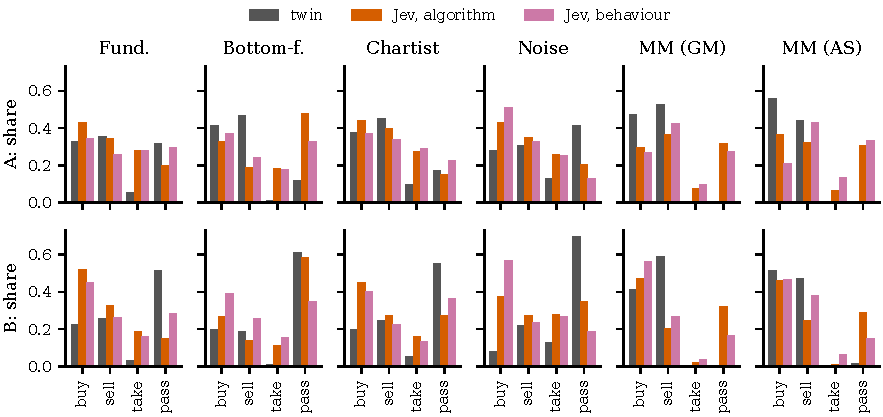
\includegraphics[width=\linewidth]{figures/stage1_shares.pdf}
\caption{Stage 1a: share of probability on buying (bid or take the ask), selling, taking (either side) and passing.}
\label{fig:sh}
\end{figure}

\input{appendix_stage2.tex}

\end{document}
